\section{Análisis}

\subsection{Listado de todas las publicaciones de un autor determinado.}

\begin{minted}[
frame=single]{js}
db.authors.aggregate([
  { $match : { _id : "Chin-Wang Tao" } }, 
  { $project: {publication: {$concatArrays: 
    ["$incollections.title", "$articles.title", "$inproceedings.title"]}}
  }
] )
\end{minted}

\subsection{Número de publicaciones de un autor determinado.}

\begin{minted}[
frame=single]{js}
db.authors.aggregate([
  { $match : { _id : "Chin-Wang Tao" } }, 
  { $project: {publication: {$concatArrays: 
    ["$incollections.title", "$articles.title", "$inproceedings.title"]}}
  },
  {$project: {number_of_publications: {$size: "$publications"}}}
] )
\end{minted}

\subsection{Número de artículos en revistas para el año 2017.}

\begin{minted}[
frame=single]{js}
db.articles.find({year: 2017}).count()
\end{minted}

En esta simple query podemos ver la importancia que adquieren los índices en cuanto a tiempo de ejecución:

\begin{figure}[H]
  \centering
    \centering
        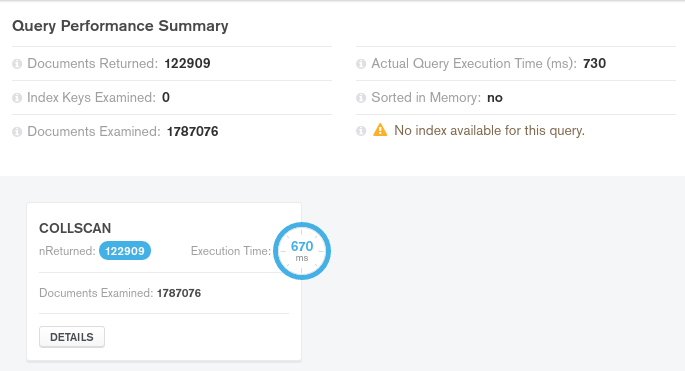
\includegraphics[width=0.4\textwidth]{Figures/wo_year_idx}
        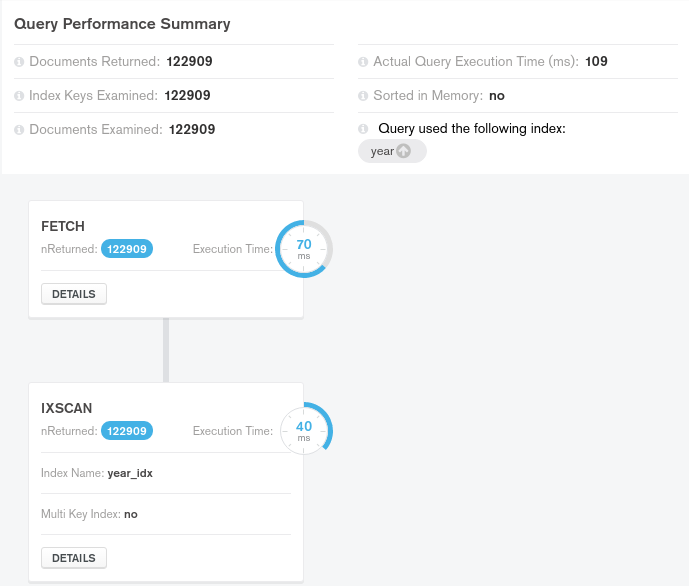
\includegraphics[width=0.4\textwidth]{Figures/year_idx}
  \caption{A la izquierda, la query sin indice, a la deracha, aplicando un índice sobre la columna year.}
\end{figure}

El tiempo de respuesta es aproximadamente 5 veces inferior al hacer uso del índice.
